\documentclass{article}
\usepackage{graphicx} % Required for inserting images
\usepackage{amsmath}
\usepackage{mathtools}
\title{Notes on thermodynamic and structural constraints in autocatalytic networks}
\author{Simone Cavallero}
\date{February 2024}
\usepackage{multicol}
\usepackage{here}

\usepackage[utf8]{inputenc}
\usepackage{biblatex} %Imports biblatex package
\addbibresource{ref.bib} %Import the bibliography file
\newcommand{\notimplies}{%
	\mathrel{{\ooalign{\hidewidth$\not\phantom{=}$\hidewidth\cr$\implies$}}}}
\begin{document}
	
	\maketitle
	
	\section{Introduction}
	Here we present the results and considerations obtained studying autocatalytic reaction examples. We'll focus in the following on explaining what it means to lose the \textbf{tight-coupling} condition and what it means to have \textbf{irreversible reactions}.
	
	\subsection{Hinshelwood cycle with tight coupling}
	When we talk about Hinshelwood Cycle we suppose a process in which we have already noticed the possibility to neglect the intermediate species, directly writing the reaction as 
	
	\\
	\begin{center}
		\newline
		$\mathrm{A} \xrightleftharpoons[j_{-1}]{j_{+1}}\mathrm{A+B}\\
		\mathrm{B} \xrightleftharpoons[j_{-2}]{j_{+2}}\mathrm{B+A}\\$
	\end{center}
	
	To have tight coupling, we assume that we chemostat or degrade just one of the two species. Following the stoichiometric framework of \cite{1} one writes:
	
	
	
	$$S=S^{-1}=
	\begin{pmatrix}
		0 & 1 \\
		1 & 0 
	\end{pmatrix}
	\ \ \ S_{+}=
	\begin{pmatrix}
		1 & 0 \\
		0 & 1 
	\end{pmatrix}
	\ \ \ S_{-}=
	\begin{pmatrix}
		1 & 1 \\
		1 & 1 
	\end{pmatrix}
	$$
	The autocatalytic mode if we chemostat species $B$ will be $$\mathbf{g}_B=\begin{pmatrix}
		0 \\ 1 
	\end{pmatrix}$$
	Thus leading to a tight coupling condition $$\begin{pmatrix}
		j_1 \\ j_2 
	\end{pmatrix}=\mathcal{J}(b) \mathbf{g}_B$$
	Hence, tight coupling condition ensures that, since we have a well defined outflow $\mathcal{J}(b)$ and $b$ is chemostat by degradation thanks to the degradation parameter $\kappa$
	$$\partial_{\kappa} \mathcal{J}(\kappa) = \partial_{\kappa} j_1 = \partial_{\kappa} j_2=0$$
	
	So that if we define $$F_{\pm i}= \partial_{\kappa} \log j_{\pm i}$$ we end up with, thanks to the maximization constraint
	
	
	\hfill \break
	
	\begin{minipage}{0.5\textwidth}
		\begin{cases}
			j_{-1}F_{-1}=j_{+1}F_{+1}\\
			j_{-2}F_{-2}=j_{+2}F_{+2}
			
		\end{cases}
	\end{minipage}
	\begin{minipage}{0.5\textwidth}
		
		\begin{cases}
			F_{-1}=F_{+1}+F_{+2}\\
			F_{-2}=F_{+1}+F_{+2} 
			
		\end{cases}
	\end{minipage}
	\hfill \break
	
	This allows the reaction's affinity to be independent of the kinetics $$
	A_1=\log \left( \frac{j_{+1}}{j_{-1}} \right)=\log \left( \frac{F_{-1}}{F_{+1}} \right)$$
	
	$$
	A_2=\log \left( \frac{j_{+2}}{j_{-2}} \right)=\log \left( \frac{F_{-2}}{F_{+2}} \right)$$
	
	This framework is general when \textbf{only one of the species is degraded by $\kappa$}, but in this specific example choosing to chemostat either species A or B will lead to the same result of a diverging optimized affinity. In fact, supposing to chemostat species B, while A is not degraded, we have tight-coupling such that
	
	\begin{center}
		\begin{cases}
			j_{-1}F_{-1}=j_{+1}F_{+1}\\
			j_{-2}F_{-2}=j_{+2}F_{+2}         
		\end{cases}
	\end{center}
	
	but since $\mathbf{g}_B= \begin{pmatrix}
		0 \\
		1
	\end{pmatrix}$ the overall affinity reads
	
	$$\mathcal{A}=\mathcal{A}_2=\log \left( \frac{F_{-2}}{F_{+2}} \right)=\log \left( 1+\frac{F_{+1}}{F_{+2}} \right)$$
	
	Optimizing this with respect to the $F$'s leads to have either $F_{+1}=0$ or $F_{+2}=0$
	
	
	\section{Beyond Tight-coupling}
	Here we present examples in which tight coupling is lost. This is due to the fact that we're going to chemostat more than one species, thus leading to have only one partial to be maximized. In the cases before, indeed, we had that if $\frac{\partial \mathcal{J}}{\partial \kappa}=0$ then $\frac{\partial j_i}{\partial \kappa}=0$ for all $i$'s in the CRN ($i=1,2$), allowing us to define the stoichiometric framework, so that the optimal affinities could have been written in terms of the $F$'s . Now, this is not possible anymore, $\frac{\partial j_i}{\partial \kappa}=0$ will be true only for some $i$'s (either $i=1$ or $i=2$, separately), depending on those species we're trying to maximize the production. Indeed, if we are chemostating more than one species we get
	
	$$\begin{pmatrix}
		j_1 \\ j_2 
	\end{pmatrix}=\mathcal{J}_A(k) \mathbf{g}_A+\mathcal{J}_B(k) \mathbf{g}_B$$
	
	This means that there's not only one single outflow to maximize, indeed we can maximize either $j_a=\kappa a$ or $j_b=\kappa b$ and thanks to the steady state equations if, for instance, we maximize $j_b$
	
	$$\partial_{\kappa} j_b = \partial_{\kappa} j_1=0 \implies j_{-1}F_{-1}=j_{+1}F_{+1}$$
	$$\partial_{\kappa} j_a = \partial_{\kappa} j_2 \neq 0 \notimplies j_{-2}F_{-2}=j_{+2}F_{+2}$$
	
	\subsection{Hinshelwood with 2 species degrading}
	Both the species are degrading with the same degradation constant $\kappa$:
	\begin{center}
		
		\hfill \break
		
		$\mathrm{A} \xrightleftharpoons[j_{-1}]{j_{+1}}\mathrm{A+B}\xrightarrow{\kappa}\emptyset\\
		\mathrm{B} \xrightleftharpoons[j_{-2}]{j_{+2}}\mathrm{B+A}\xrightarrow{\kappa}\emptyset\\
		$
		
		
	\end{center}
	Solving the steady state equations: 
	\hfill \break
	\hfill \break
	\begin{center}
		
		\begin{cases}
			j_1-j_b =0 \\ j_2-j_a=0
		\end{cases}
	\end{center}
	
	
	with \\
	\begin{center}
		\begin{cases}
			j_1=k_{+1}a-k_{-1}ab \\   j_2=k_{+2}b-k_{-2}ab   \\  j_a=\kappa a \\ j_b=\kappa b
		\end{cases}
	\end{center}
	
	\hfill \break
	The optimal affinities read
	$$A_1^*=\log \left( \frac{b_{eq}}{b^*} \right)$$
	$$A_2^*=\log \left( \frac{a_{eq}}{a^*} \right)$$
	
	Considering to maximize the production of the $B$ species, we ask for $\frac{\partial j_b}{\partial k}=\frac{\partial j_1}{\partial k}=0$, leading to two results:
	\begin{center}
		$$\frac{\partial}{\partial k} \log b = -\frac{1}{k}$$
		
		$$\frac{j_{+1}}{j_{-1}}=\frac{F_{-1}}{F_{+1}} \ \ \implies \ \ A_1^*=\log \left( \frac{F_{-1}^*}{F_{+1}^*} \right) $$
	\end{center}
	
	So that we obtain a definition of $A_1$ which is independent of kinetics. Plotting $A_1^*$ and $A_2^*$
	we end up with the following relations:
	
	\begin{figure}[h!]
		
		\begin{subfigure}{\textwidth}
			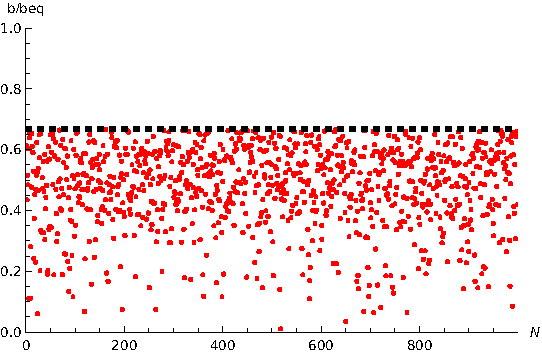
\includegraphics[width=0.45\linewidth]{plot.pdf}
		\end{subfigure}
		\begin{subfigure}{\textwidth}
			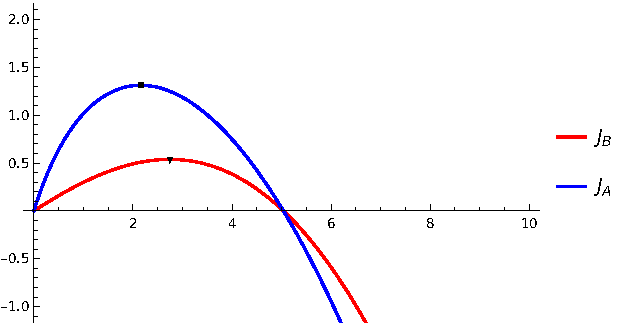
\includegraphics[width=0.45\linewidth]{plotJ.pdf}
		\end{subfigure}
	\end{figure}
	\hfill
	\begin{figure}[h!]
		\begin{subfigure}{ \textwidth}
			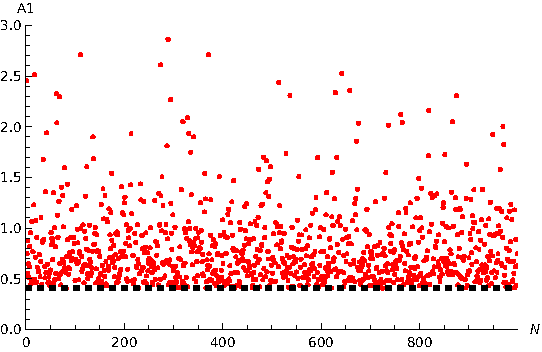
\includegraphics[width=0.45\linewidth]{plotA1.pdf}
		\end{subfigure}
		\begin{subfigure}{ \textwidth}
			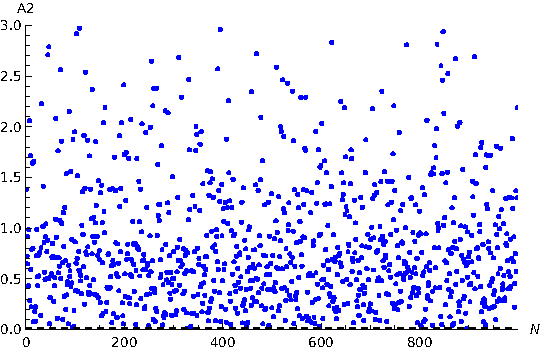
\includegraphics[width=0.45\linewidth]{plotA2.pdf}
		\end{subfigure}
	\end{figure}
	\hfill
	\begin{figure}[h!]
		\begin{subfigure}{\textwidth}
			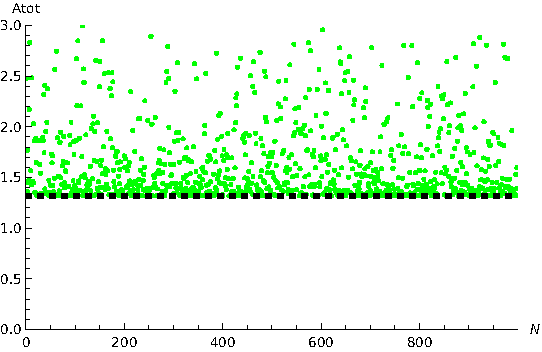
\includegraphics[width=0.45\linewidth]{plotA1A2.pdf}
		\end{subfigure}
		\begin{subfigure}{\textwidth}
			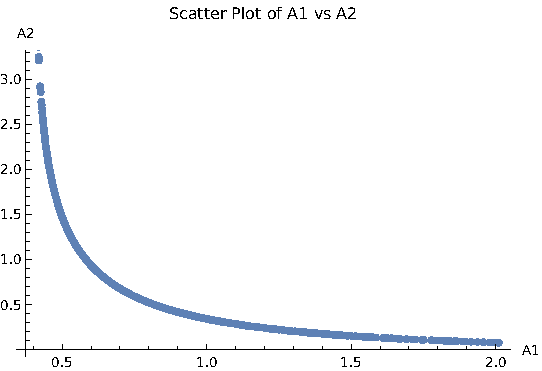
\includegraphics[width=0.45\linewidth]{Arel.pdf}
		\end{subfigure}
	\end{figure}
	
	
	
	
	
	
	Stating important bounds and results:
	\begin{itemize}
		\item $\frac{b^*}{beq} \le \frac{2}{3}$
		\item $A_1^* \ge \log \frac{3}{2}$ (equivalent to the one above)
		\item $A_2^* \ge 0$ (trivial)
		\item $A_1^*+A_2^* \ge \log  3.73  \ \ \text{(don't know why)}$
		\item $A_1^*$ and $A_2^*$ are deeply linked by a constraint
		
		
	\end{itemize}
	
	\subsection{Hinshelwood with 3 or 4 species degrading}
	
	Considering higher number of species always following Hinshelwood patter such as
	
	\begin{center}
		$\mathrm{A} \xrightleftharpoons[j_{-1}]{j_{+1}}\mathrm{A+B}\xrightarrow{\kappa}\emptyset\\
		\mathrm{B} \xrightleftharpoons[j_{-2}]{j_{+2}}\mathrm{B+C}\xrightarrow{\kappa}\emptyset\\
		\mathrm{C} \xrightleftharpoons[j_{-3}]{j_{+3}}\mathrm{C+A}\xrightarrow{\kappa}\emptyset\\
		$
	\end{center}
	
	And supposing to maximize the current of the last species $C$ one obtains
	
	\begin{itemize}
		\item $\frac{c^*}{ceq} \le \frac{3}{4}$
		\item $A_2^* \ge \log \left( \frac{4}{3}\right)$
		\item $A_1^*, A_3^* \ge 0$
		
		\item $A_1^*$-$A_2^*$ and $A_3^*$-$A_2^*$ are deeply linked by a constraint (an inequality)
	\end{itemize}
	
	For the 4 species case the pattern becomes visible
	
	\begin{center}
		$\mathrm{A} \xrightleftharpoons[j_{-1}]{j_{+1}}\mathrm{A+B}\xrightarrow{\kappa}\emptyset\\
		\mathrm{B} \xrightleftharpoons[j_{-2}]{j_{+2}}\mathrm{B+C}\xrightarrow{\kappa}\emptyset\\
		\mathrm{C} \xrightleftharpoons[j_{-3}]{j_{+3}}\mathrm{C+D}\xrightarrow{\kappa}\emptyset\\
		\mathrm{D} \xrightleftharpoons[j_{-4}]{j_{+4}}\mathrm{D+A}\xrightarrow{\kappa}\emptyset\\
		$
	\end{center}
	
	And supposing to maximize the current of the last species $D$ one obtains
	
	\begin{itemize}
		\item $\frac{d^*}{deq} \le \frac{4}{5}$
		\item $A_3^* \ge \log \left( \frac{5}{4}\right)$
		\item $A_1^*, A_2^*, A_4^* \ge 0$
		
		
	\end{itemize}
	
	\subsection{Hinshelwood with MM degradation for the maximized species}
	
	The model in this case is the same as before, for 2 species, besides the degradation of the species which we are going to maximize is set to be of the simplified MM type
	
	\begin{center}$\mathrm{A} \xrightleftharpoons[j_{-1}]{j_{+1}}\mathrm{A+B}\xrightarrow{\kappa}\emptyset\\
		\mathrm{B} \xrightleftharpoons[j_{-2}]{j_{+2}}\mathrm{B+A}\xrightarrow{\kappa}\emptyset\\
		$
	\end{center}
	The evolution equations read
	
	\begin{equation}
		\frac{da}{dt}=k_{+2}b -k_{-2}ab - \kappa a
	\end{equation}
	\begin{equation}
		\frac{db}{dt}=k_{+1}a -k_{-1}ab - \kappa \frac{b}{1+b}
	\end{equation}
	
	with 
	
	\begin{equation}
		j_1=k_{+1}a -k_{-1}ab 
	\end{equation}
	\begin{equation}
		j_2=k_{+2}b -k_{-2}ab
	\end{equation}
	\begin{equation}
		j_a=\kappa a
	\end{equation}
	\begin{equation}
		j_b=\kappa \frac{b}{1+b} 
	\end{equation}
	
	The steady states concentrations read
	
	$$a_{ss}=\frac{\kappa ^2 k_{-2}+\kappa  \sqrt{\left(\kappa  k_{-2}+k_{-1} k_2-k_1 k_2\right){}^2-4 k_{-1} k_2 \left(\kappa ^2-k_1 k_2\right)}-\kappa  k_{-1} k_2+\kappa  k_1 k_2-2 k_{-2} k_1 k_2}{2 \left(\kappa ^2 k_{-1}-\kappa  k_{-2} k_{-1}+\kappa  k_{-2} k_1-k_{-2}^2 k_1\right)}$$
	
	$$b_{ss}=\frac{\sqrt{\left(\kappa  k_{-2}+k_{-1} k_2-k_1 k_2\right){}^2-4 k_{-1} k_2 \left(\kappa ^2-k_1 k_2\right)}-\kappa  k_{-2}-k_{-1} k_2+k_1 k_2}{2 k_{-1} k_2}$$
	
	Being analytically too complex to study, we can see numerically what the bound on $\frac{b}{b_{eq}}$ look like in these conditions
	
	
	\begin{figure}[h!]
		\centering
		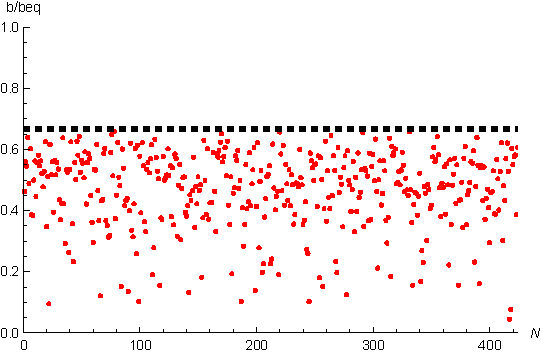
\includegraphics[width=0.45\linewidth]{MM.pdf}
	\end{figure}
	
	
	\subsection{Irreversibility in the Hinshelwood cycle}
	Considering all the reactions to be irreversible, no matter the scale of the cycle, we always end up with steady states of zero concentrations for all the species, differently from the prey-predator results. Hence, the model is not interesting neither structurally nor thermodynamically when the reactions are set to be irreversibile. We leave this section open for possible fluxes and typical times analysis, which may be relevant from an experimental point of view.
	
	
	
	\section{Prey-predator model}
	In the following, we will assume a prey-predator model with Michaelis-Menten reproduction for the prey production and Mass Action Law for the predation and analyze its characteristics.
	
	\subsection{Linear degradation for both species} \label{MMNOREV}
	The model from \cite{2} is a classic prey-predator with both the species degrading with different rates:
	
	\begin{center}
		$\mathrm{N} \rightarrow\mathrm{2N}\\
		\mathrm{N+P} \rightarrow 2P\\
		N  \rightarrow \emptyset\\
		P \rightarrow \emptyset$
	\end{center}
	
	The first dynamics we studied has been done with linear degradation, no backwards reactions and Michaelis-Menten for preys evolution:
	
	\begin{equation}
		\frac{dn}{dt}=\frac{gn}{1+\beta g n}-n p-\lambda \delta n
	\end{equation}
	\begin{equation}
		\frac{dp}{dt}=n p-\delta p
	\end{equation}
	
	We take the steady state that corresponds to both preys and predator $\neq 0$ and we maximize the degradation current for the predators (i.e. $\deltap$). Since we can't define any thermodynamic quantity, we notice bounds for the optimal concentration:
	
	$$\frac{p^*}{p_{eq}}\le \frac{1}{2}$$
	
	This bound results to be independent from:
	\begin{itemize}
		\item the degradation type (linear or non linear)
		\item MAL or MM for the preys
		\item reversibility of the reactions
		
	\end{itemize}
	
	\textbf{NOTE:} We managed to prove, from dynamics and kinetics, the bound in different cases, whether it follows MM or MAL, with the first reaction to be reversible and also when the degradation is nonlinear, but the framework doesn't seem to be that general.
	
	\subsubsection{Dynamical analysis for linear degradation}
	The relevant steady state of the system is:
	$$\begin{pmatrix}
		n_{ss} \\ p_{ss}
	\end{pmatrix}=\begin{pmatrix}
		\delta \\ \frac{g}{1+g \beta \delta}-\lambda \delta
	\end{pmatrix} $$
	
	with
	$$ \begin{pmatrix}
		n_{eq} \\ p_{eq}
	\end{pmatrix}=\begin{pmatrix}
		0 \\ g
	\end{pmatrix} $$
	
	Asking for the maximization of the predator outflow $j_p=\delta*p$
	
	$$\partial_{\delta}(\delta p)=0 \implies \partial_{\delta} \log p^*=-\frac{1}{\delta}$$
	
	In this case, giving
	
	$$\frac{\lambda (1+2\beta g \delta)}{p (1+\beta g \delta)} + \frac{\beta g}{1+ \beta g \delta}=\frac{1}{\delta} 
	\ \ \ \Longleftrightarrow$$$$
	\lambda \delta= \frac{p}{1+2\beta g \delta}$$
	
	But we know $p$ from steady state, so that we can substitute $\lambda \delta $
	
	$$p=\frac{g}{1+ \beta g \delta }-\frac{p}{1+ 2 \beta g \delta }
	\ \ \  \Longleftrightarrow$$$$
	p=\frac{g}{2}  \frac{1+2x}{(1+x)^2} \le \frac{g}{2}=\frac{p_{eq}}{2}$$
	
	with $x= \beta g \delta$
	
	\subsection{Non-Linear degradation for the maximized species}
	The model can be generalized to have non-linear degradation for both preys and predators. Adding it only to preys one has:
	
	\begin{equation}
		\frac{dn}{dt}=\frac{g n}{1+\beta g n}-n p-\lambda \delta n
	\end{equation}
	\begin{equation}
		\frac{dp}{dt}=n p-\delta \frac{p}{1+p}
	\end{equation}
	
	As stated before, the model, when there is a stable fixed point leading to a steady state, still respects the upper bound on the concentration $p^*$ when its outgoing current is maximized. But this model can present an oscillating regime for some values of the parameters. Necessary conditions to have oscillations, a priori from the choice of the parameters are:
	
	\begin{itemize}
		\item MM for the first reaction
		\item non-linear degradation at least for the preys
	\end{itemize}
	
	\subsubsection{Linear Stability Analysis for the Non-linear degradation}
	One could then use Linear Stability Analisys to study the region of oscillations, exploiting the properties of the Jacobian. 
	
	$$J= \begin{pmatrix}
		g-2\beta g^2 n_{ss}-p_{ss}-\lambda \delta & -n_{ss}\\ p_{ss} & n_{ss}-\frac{\delta}{1+p_{ss}}
	\end{pmatrix}$$
	
	If we want to study where the Hopf Bifurcation occurs, the $Tr(J)$ has to change sign, this occurs when
	
	$$n_{ss}(1-2 \beta  g^2)-p_{ss}-\frac{\delta}{(1+p_{ss})^2}=\lambda \delta -g$$
	
	Fixing $\beta=0.087$ and $\delta=0.39$ as has been done in Yannick's paper \cite{2}, we obtain the following graph for the relation ($\lambda - \delta)$, which seems to agree with what has been obtained by them:
	
	\hfill \break 
	
	\begin{figure}[h!]
		
		\begin{subfigure}{\textwidth}
			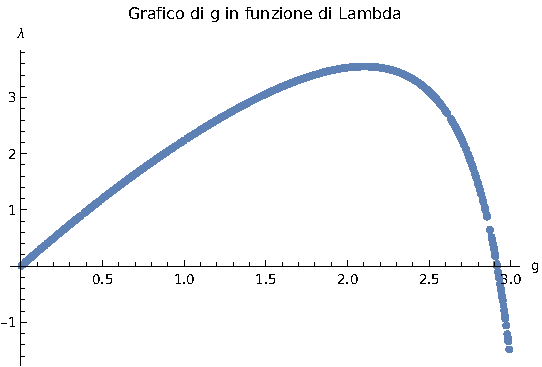
\includegraphics[width=0.45\linewidth]{plotPP.pdf}
		\end{subfigure}
		\begin{subfigure}{\textwidth}
			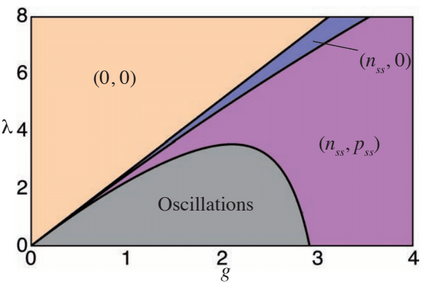
\includegraphics[width=0.45\linewidth]{Yan.png}
		\end{subfigure}
	\end{figure}
	If we ask for the maximization of the current i.e. $\partial_{\delta} (\delta \frac{p}{1+p})=0$, a feature we introduce, we can only do it for the purple part, because there we have an analytic expression for the steady state. This results in
	
	
	\begin{figure}[H]
		\begin{center}
			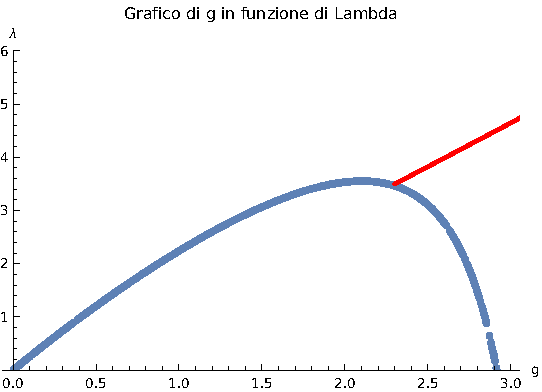
\includegraphics[width=0.4\linewidth]{plotmax.pdf}
		\end{center}
	\end{figure}
	
	This means that moving on the red line, from the stable point regime to the oscillations one, we can study how the stable point opens into a limit cycle, to notice the behaviour of this with respect to the bound:
	
	\hfill \break
	
	\begin{figure}[H]
		
		\begin{subfigure}{\textwidth}
			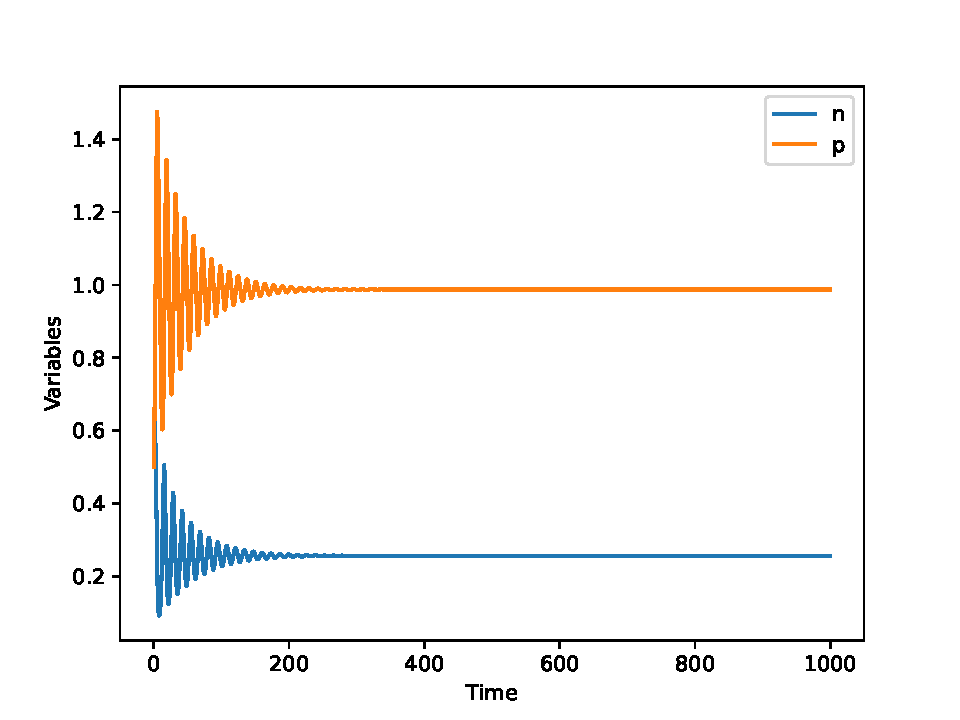
\includegraphics[width=0.5\linewidth]{timeseries.pdf} 
		\end{subfigure}
		\begin{subfigure}{\textwidth}
			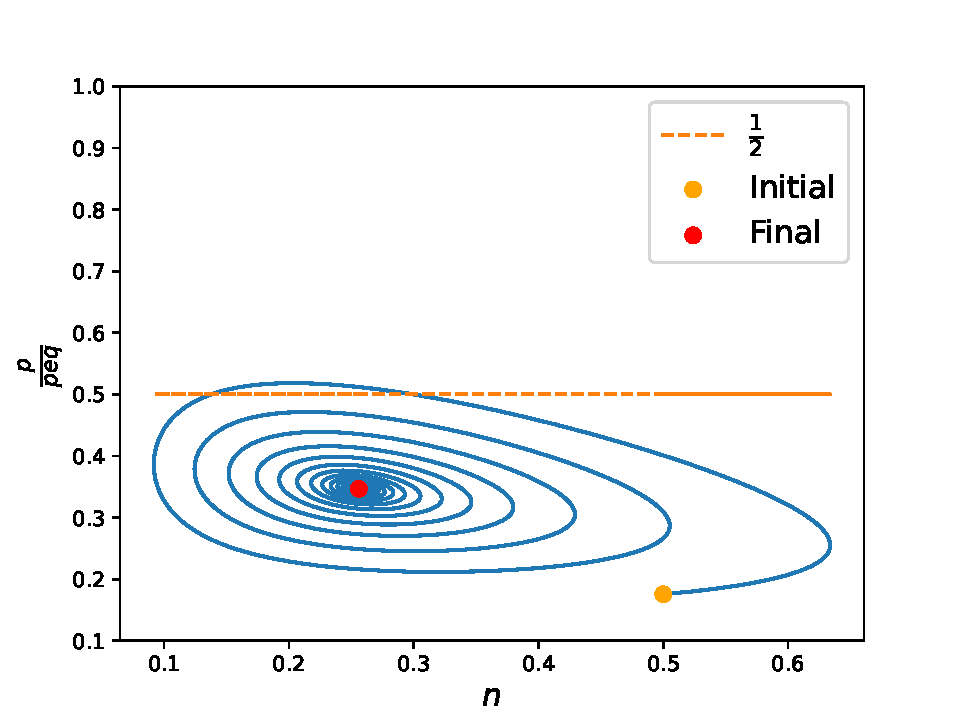
\includegraphics[width=0.5\linewidth]{traj.pdf} 
		\end{subfigure}
		\caption{\small{Time series and Trajectory for values of $g$ and $\lambda$  close to the Hopf Bifurcation but still in the stable regime}}
	\end{figure}
	\begin{figure}[H]
		\begin{subfigure}{\textwidth}
			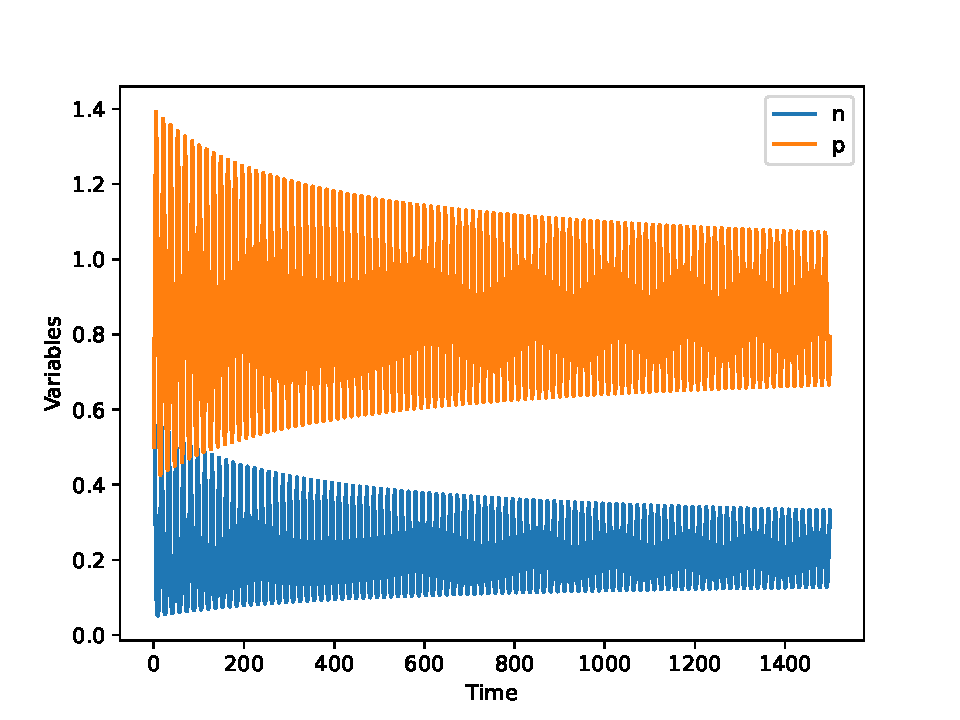
\includegraphics[width=0.5\linewidth]{timeseries1.pdf}
		\end{subfigure}
		\begin{subfigure}{\textwidth}
			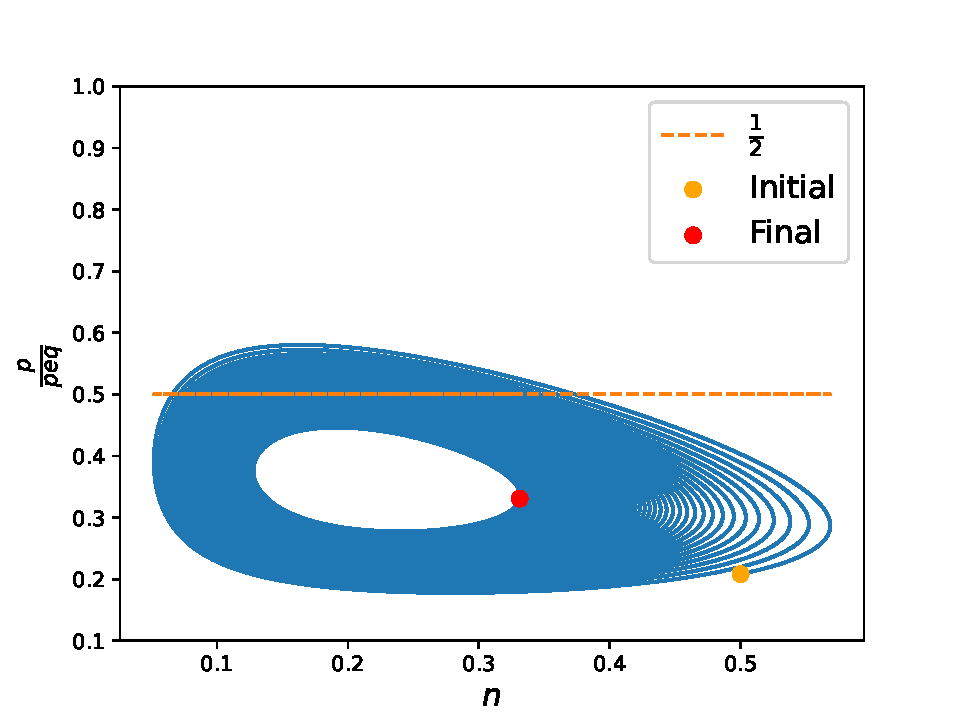
\includegraphics[width=0.5\linewidth]{traj1.pdf}
		\end{subfigure}
		\caption{\small{Time series and Trajectory for values of $g$ and $\lambda$  close to the Hopf Bifurcation but already in the oscillating regime}}
	\end{figure}
	Moreover, one could study, for the same values of $\beta$ and $\delta$ fixed, how max and min value of $p^*$ evolves changing $g$ (and thus changing $\lambda$ once we ask for current maximization):
	\begin{figure}[h!]
		\begin{center}
			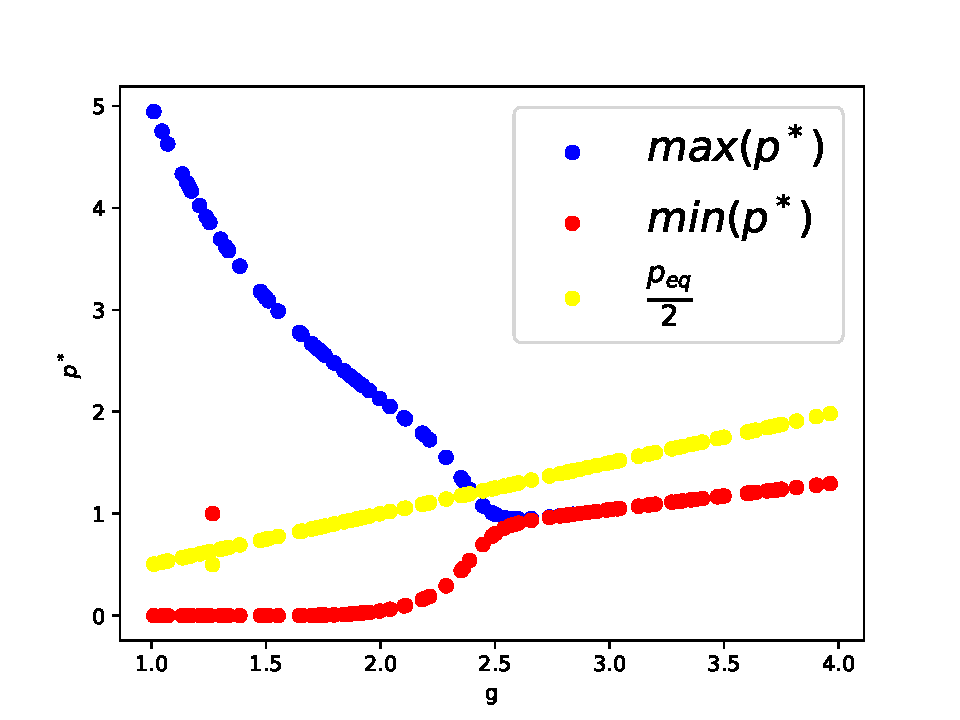
\includegraphics[width=0.7\linewidth]{LC.pdf}
		\end{center}
	\end{figure}
	
	\hfill \break
	This way, we can see the appeareance of the Limit Cycle, when we ask for the maximization of the outflow of $p$. As we can see, when the system is following a stable steady state (for high enough $g$ and $\lambda$), its optimal concentration lies below the $\frac{p_{eq}}{2}$ line, whereas it's difficult to understand how the time average of the oscillation behaves when we enter the LC case.
	
	\subsection{MAL for the entire system and reversibility for just the preys reproduction}
	We can now think of the model as having MAL and reversibility for the preys evolution (the second reaction remains irreversible)
	
	\begin{equation}
		\frac{dn}{dt}=k_{+1} n -k_{-1}n^2  -n p-\lambda \delta n
	\end{equation}
	\begin{equation}
		\frac{dp}{dt}=n p-\delta p
	\end{equation}
	
	The non trivial steady state is 
	
	$$\begin{pmatrix}
		n_{ss} \\ p_{ss}
	\end{pmatrix}=\begin{pmatrix}
		\delta \\ k_{+1}-\delta (\lambda + k_{-1})
	\end{pmatrix} $$
	
	$$ \begin{pmatrix}
		n_{eq} \\ p_{eq}
	\end{pmatrix}=\begin{pmatrix}
		0 \\ k_{+1}
	\end{pmatrix} $$
	
	The maximization condition rephrases
	
	$$ \partial_{\delta} \log p^*=-\frac{1}{\delta} \implies \delta(\lambda+ k_{-1})=\frac{k_{+1}}{2} $$
	
	So that
	
	$$p^*=k_{+1}-\frac{k_{+1}}{2}=\frac{p_{eq}}{2}$$
	
	
	\subsection{MAL for the entire system and reversibility for both the reactions} \label{MALREV}
	Let's consider the general case of the model following MAL with reversibility
	
	\begin{equation}
		\frac{dn}{dt}=k_{+1}n-k_{-1}n^2-k_{+2}n p+k_{-2}p^2-\lambda \delta n
	\end{equation}
	\begin{equation}
		\frac{dp}{dt}=k_{+2}n p-k_{-2}p^2-\delta p
	\end{equation}
	
	The dynamics of this model is quite heavy, this is the reason why it is interesting to notice some bounds directly from a stoichiometric point of view:
	
	\begin{center}
		\begin{cases}
			F_{+1}=\partial_{\delta} \log n \\
			F_{-1}=\partial_{\delta} \log n^2=2 F_{+1}\\
			F_{+2}=\partial_{\delta} \log n+\partial_{\delta} \log p\\
			F_{-2}=\partial_{\delta} \log p^2=2(F_{+2}-F_{+1})\\
		\end{cases}
	\end{center}
	The maximization condition gives
	
	$$\partial_{\delta} \log p^*=-\frac{1}{\delta} \implies \frac{F_{-2}}{2}=-\frac{1}{\delta}\implies F_{-2} \le 0 \implies F_{+1} \ge F_{+2}$$
	
	Moreover, $$\partial_{\delta}(\delta p)=\partial_{\delta} j_2=0 \implies A_2= \log \left( \frac{F_{-2}}{F_{+2}}\right)=\log \left( \frac{F_{+2}-F_{+1}}{F_{+2}}\right)+\log2$$
	
	To make the affinity to exist, we'd need $\frac{F_{+2}-F_{+1}}{F_2} >0$ but since $F_{+1} \ge F_{+2}$ this means
	
	$$F_2 \le 0$$
	
	This means that we have two possibilities
	
	\begin{center}
		\begin{cases}
			F_{+1} \ge 0 \ \Longleftrightarrow \  A_2^* \ge \log 2\\
			F_{+1} \le 0 \ \Longleftrightarrow \ A_2^* \le \log 2
		\end{cases}
	\end{center}
	
	Simulations show that, indeed, is the second case to be the one
	
	\begin{figure}[H]
		\begin{center}
			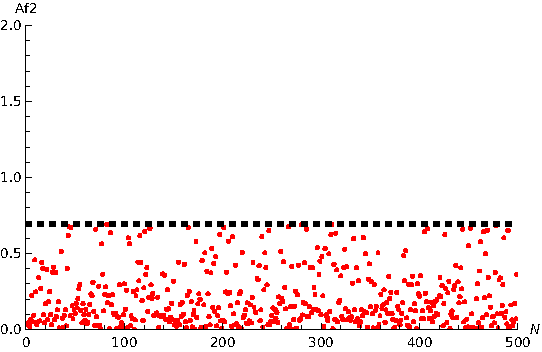
\includegraphics[width=0.5\linewidth]{
				A2PP.pdf}
		\end{center}
	\end{figure}
	
	Can we say anything for $A_1$ even though we don't have tight coupling?
	From steady state we know
	
	\begin{center}
		\begin{cases}
			j_1-j_2=\lambda \delta n\\
			j_2=\delta p
		\end{cases}
	\end{center}
	
	Eliminating $\delta$, and taking the logarithms of both sides
	
	$$\log j_2- \log p = \log (j_1-j_2)- \log (\lambda n)$$
	
	Differentiating both sides by $\delta$
	
	$$- \partial_{\delta} \log p = \partial_{\delta} \log (j_1-j_2)- \partial_{\delta} \log n \Longleftrightarrow $$
	
	$$\partial_{\delta} \log (j_1-j_2) = 2 F_{+1} - F_{+2} \implies \frac{\partial_{\delta}j_1}{j_1-j_2}=2 F_{+1} - F_{+2}$$
	
	which means $$\partial_{\delta}j_1=(j_1-j_2)(2F_{+1}-F_{+2})$$
	
	Remember that, from steady state, $j_1-j_2=\lambda \delta n >0$, and since $F_{+1}-F_{+2} \ge 0$ it has to be that
	
	$$\partial_{\delta}j_1 \ge 0$$
	
	This means that $$\frac{j_{+1}}{j_{-1}} \ge \frac{F_{-1}}{F_{+1}}$$
	
	Thus
	\begin{center}
		\begin{cases}
			F_{+1} \ge 0 \ \Longleftrightarrow \ \frac{j_{+1}}{j_{-1}} \ge 2 \implies A_1^* \ge \log 2\\
			F_{+1} \le 0 \ \Longleftrightarrow \ \frac{j_{+1}}{j_{-1}} \le 2 \implies A_1^* \le \log 2\\
		\end{cases}
	\end{center}
	
	Again, simulations show the second case to be the fulfilled one
	
	\begin{figure}[H]
		\begin{center}
			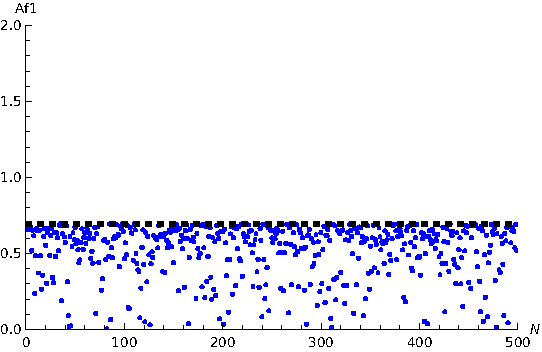
\includegraphics[width=0.5\linewidth]{
				A1PP.pdf}
		\end{center}
	\end{figure}
	
	
	
	\section{Sensitivity considerations}
	Inspired by Horowitz paper \cite{3} on the sensitivity of the average values of quantities with respect to parameters of the model, we saw that, in his framework of a Markov Process he proved:
	
	\begin{equation}
		\left|\frac{d \log \frac{\langle A \rangle}{\langle B \rangle} }{d \log \kappa}\right| \le m 
	\end{equation}
	where $m$ is the size of the support for the parameter $\kappa$, i.e. an integer indicating how many nodes (species) evolution depend on the parameter $\kappa$ in the CRN corresponding graph (See \cite{3}). Note that this bound is independent from the quantities $A$ and $B$, the only important thing is that these two quantities fluctuate in the stochastic system. $\kappa$ is whatever parameter of the system (rate constants, degradation constant, parameter of MM...). We asked ourselves whether this bound may hold, with a similar prove, in our deterministic case.
	
	\subsection{Hinshelwood's sensitivity}
	
	\begin{center}
		\begin{equation}
			\mathrm{A} \xrightleftharpoons[j_{-1}]{j_{+1}}\mathrm{A+B}\xrightarrow{\kappa}\emptyset\\
			\mathrm{B} \xrightleftharpoons[j_{-2}]{j_{+2}}\mathrm{B+A}\xrightarrow{\kappa}\emptyset\\
		\end{equation}
	\end{center}
	
	Before asking for the maximization of the outflow of $B$, we notice that
	\begin{equation}
		\frac{d \log \frac{ a}{b} }{d \log \kappa}=\kappa \partial_{\kappa} \log \frac{ a }{b} 
	\end{equation}
	The steady state for Hinshelwood cycle reads:
	
	$$a_{ss}=\frac{k_{+1}k_{+2}-\kappa^2}{\kappa k_{-1}+k_{-2}k_{+1}}$$
	$$b_{ss}=\frac{k_{+1}k_{+2}-\kappa^2}{\kappa k_{-2}+k_{-1}k_{+2}}$$
	
	Hence
	
	$$\frac{a_{ss}}{b_{ss}}=\frac{\kappa k_{-2}+k_{-1}k_{+2}}{\kappa k_{-1}+k_{-2}k_{+1}}$$
	
	It's important to notice that \textbf{both numerator and denominator have positive terms in the sum}. This is what will allow us to define the bound during this calculation
	
	$$\kappa \partial_{\kappa}\log \left( \frac{a_{ss}}{b_{ss}}\right)=\frac{\kappa k_{-2}}{\kappa k_{-2}+k_{-1}k_{+2}}- \frac{\kappa k_{-1}}{\kappa k_{-1}+k_{-2}k_{+1}}$$
	
	It's easy to notice that both the terms on right-hand side are bounded in the interval $[0,1]$. Thus
	
	$$\kappa \partial_{\kappa}\log \left( \frac{a_{ss}}{b_{ss}}\right) \in [-1,1]$$
	
	Recovering an $m=1$ (we would have expected $m=2$ for the support...). We notice that the proof for this bound is indeed very similar to what has been done by Horowitz \cite{3}. We will abuse of notation for $a$ and $a_{ss}$ or $b$ and $b_{ss}$ knowing we're talking about the same quantity
	
	Now inserting the maximization condition 
	
	\begin{equation}
		\partial_{\kappa}\log b=-\frac{1}{\kappa}
	\end{equation}
	
	we have
	
	$$\kappa \partial_{\kappa}\log \left( \frac{a_{ss}}{b_{ss}}\right)=\kappa (\partial_{\kappa} \log a - \partial_{\kappa} \log b)=\kappa\partial_{\kappa} \log a-1 \in [-1,1]$$
	
	so that
	
	\begin{equation}
		-\kappa \partial_{\kappa} \log a\in [0,2]
	\end{equation}
	
	and 
	
	\begin{equation}
		\frac{1}{-\kappa \partial_{\kappa} \log a}\in \left[\frac{1}{2},+\infty\right)
	\end{equation}
	
	We remind that the optimal affinity, inserting the maximization condition $$A_1^*=\log\left(\frac{F_{-1}}{F_{+1}}\right)=\log\left(1+\frac{\partial_{\kappa}\log b}{\partial_{\kappa}\log a}\right)=\log\left(1+\frac{1}{-\kappa \partial_{\kappa}\log a}\right)$$
	
	So that, for what just proven above,
	
	$$A_1^* \ge \log \frac{3}{2}$$
	
	
	\begin{figure}[H]
		\begin{center}
			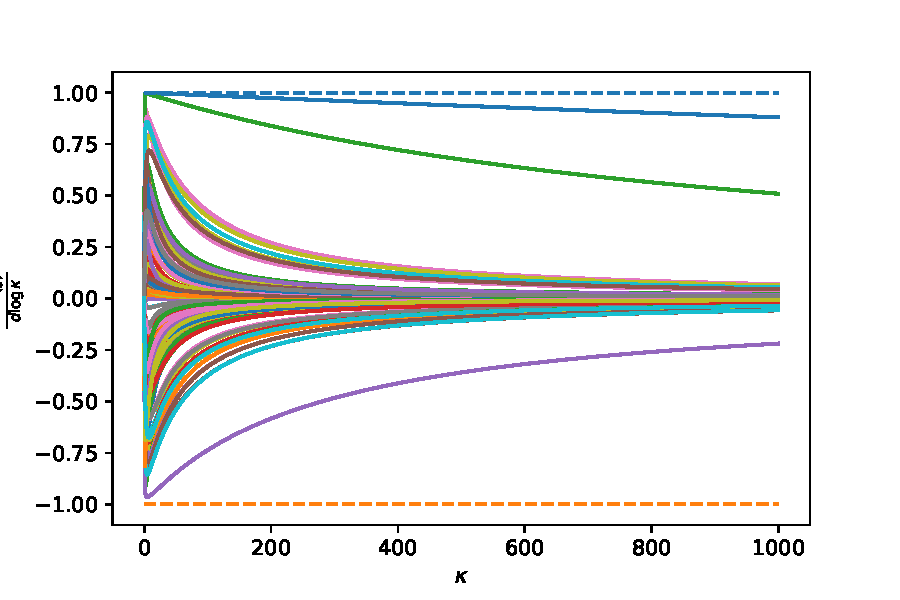
\includegraphics[width=0.7\linewidth]{sens.pdf}
			\caption{Log-sensitivity of the ratio $\frac{a}{b}$ with many realizations of the rate constants}
		\end{center}
	\end{figure}
	
	The same process can be generalized for larger Hinshelwood networks.
	
	\begin{center}
		\begin{equation}
			\mathrm{A} \xrightleftharpoons[j_{-1}]{j_{+1}}\mathrm{A+B}\xrightarrow{\kappa}\emptyset\\
			\mathrm{B} \xrightleftharpoons[j_{-2}]{j_{+2}}\mathrm{B+C}\xrightarrow{\kappa}\emptyset\\
			\mathrm{C} \xrightleftharpoons[j_{-3}]{j_{+3}}\mathrm{C+A}\xrightarrow{\kappa}\emptyset\\
		\end{equation}
	\end{center}
	
	Again, if for 3-Hinsh we ask to maximize, without loss of generality, the outflow of $B$, then is again
	
	$$\partial_{\kappa}(j_b)=0 \implies \partial_{\kappa}(j_1)=0 \implies \frac{j_{+1}}{j_{-1}}=\frac{F_{-1}}{F_{+1}}$$
	
	Then
	
	$$A_1^*=\log\left(\frac{F_{-1}}{F_{+1}}\right)=\log\left(1+\frac{\partial_{\kappa}\log b}{\partial_{\kappa}\log a}\right)=\log\left(1+\frac{1}{-\kappa \partial_{\kappa}\log a}\right)$$
	
	The steady states now read
	
	$$a_{ss}=\frac{k_1 k_2 k_3-\kappa ^3}{\kappa ^2 k_{-1}+\kappa  k_{-2} k_1+k_{-3} k_1 k_2} \ \ \ b_{ss}=\frac{k_1 k_2 k_3-\kappa ^3}{\kappa ^2 k_{-2}+\kappa  k_{-3} k_2+k_{-1} k_2 k_3}$$ $$c_{ss}=\frac{k_1 k_2 k_3-\kappa ^3}{\kappa ^2 k_{-3}+\kappa  k_{-1} k_3+k_{-2} k_1 k_3}$$
	
	We need to calculate, for the Horowitz bound
	
	\begin{equation}
		\frac{d \log \frac{ a}{b} }{d \log \kappa}=\kappa \frac{d \log \frac{ a }{b} }{d\kappa}
	\end{equation}
	
	One has 
	
	$$\frac{a}{b}=\frac{\kappa ^2 k_{-2}+\kappa  k_{-3} k_2+k_{-1} k_2 k_3}{\kappa ^2 k_{-1}+\kappa  k_{-2} k_1+k_{-3} k_1 k_2}$$
	
	$$\kappa \partial_{\kappa}\log \frac{a}{b}= \frac{2 \kappa ^2 k_{-2}+\kappa  k_{-3} k_2+k_{-1} k_2 k_3}{\kappa ^2 k_{-2}+\kappa  k_{-3} k_2+k_{-1} k_2 k_3} -  \frac{2 \kappa ^2 k_{-1}+\kappa  k_{-2} k_1+k_{-3} k_1 k_2}{\kappa ^2 k_{-1}+\kappa  k_{-2} k_1+k_{-3} k_1 k_2} $$
	
	As before, it's easy to notice that the two terms on the right-hand side are bounded in the interval $[0,2]$ thus giving
	
	$$\left|\kappa \partial_{\kappa}\log \frac{a}{b}\right| \le 2 $$
	
	with $m=2$. Inserting the maximization condition again
	
	$$\kappa \partial_{\kappa}\log \left( \frac{a}{b}\right)=\kappa (\partial_{\kappa} \log a - \partial_{\kappa} \log b)=\kappa\partial_{\kappa} \log a-1 \in [-2,2]$$
	
	\begin{equation}
		-\kappa \partial_{\kappa} \log a\in [-1,3]
	\end{equation}
	
	or 
	
	\begin{equation}
		-\frac{1}{\kappa \partial_{\kappa} \log a} \in \left(-\infty ,-1\right] \cup \left[ \frac{1}{3}, +\infty \right)
	\end{equation}
	
	Again, this leads to 
	
	$$A_1^* \ge \log \frac{4}{3}$$
	
	The same arguments work for larger Hinshelwood networks: the value of $m$ increases linearly with the number of species involved.
	
	\subsection{Prey-Predator model}
	The general model with MAL and reversibility (Sec. \ref{MALREV}), doesn't allow to get an easy insight on the Horowitz bound, because the steady state and the ratio $\frac{n}{p}$ get too complex.
	
	\hfill \break
	
	It can be anyway calculated for the irreversible case with MM for the preys production (Sec. \ref{MMNOREV}) \textbf{with linear degradation}:
	\\
	
	\begin{minipage}{0.5 \textwidth}
		\begin{center}
			$\mathrm{N} \rightarrow\mathrm{2N}\\
			\mathrm{N+P} \rightarrow 2P\\
			N  \rightarrow \emptyset\\
			P \rightarrow \emptyset$
		\end{center}
		
	\end{minipage}
	\begin{minipage}{0.5 \textwidth}
		\begin{cases}
			\frac{dn}{dt}=\frac{gn}{1+\beta g n}-n p-\lambda \delta n
			\\
			\frac{dp}{dt}=n p-\delta p
		\end{cases}
	\end{minipage}
	
	\hfill \break
	
	We can then calculate
	
	$$\frac{d \log \frac{ n}{p} }{d \log \delta}=\delta \frac{d \log \frac{ n }{p} }{d\delta}$$
	
	
	Remembering the steady states 
	
	$$n_{ss}=\delta$$
	$$p_{ss}=\frac{g}{\beta  \delta  g+1}-\delta  \lambda$$
	
	So that
	
	$$\log \frac{n}{p}=\log \left( \frac{\delta }{\frac{g}{\beta  \delta  g+1}-\delta  \lambda }\right)=\log \left(\frac{\delta( \beta  \delta  g+1) }{g-\delta  \lambda (\beta  \delta  g+1) }\right)$$
	
	$$\delta \partial_{\delta}\log \frac{n}{p}=\delta \frac{1+2\beta g \delta}{\delta (1+\beta g \delta)}- \frac{-\lambda \delta (1+2\beta g \delta)}{g- \lambda \delta (1+ \beta g \delta)}=\frac{1+2\beta g \delta}{1+\beta g \delta}-\lambda \frac{n}{p}\frac{ 1+2\beta g \delta}{ 1+ \beta g \delta}$$
	
	But since $-\lambda \frac{n}{p}= - \lambda \frac{ \delta (1+ \beta g \delta)}{g-\lambda \delta (1+ \beta g \delta)} \in [0,1]$ then we have 
	$$\frac{1+2\beta g \delta}{1+\beta g \delta} \in [1,2]$$
	$$-\lambda \frac{n}{p}\frac{ 1+2\beta g \delta}{ 1+ \beta g \delta} \in [0,2]$$
	
	Meaning that, differently from a single $m$, we find a bound of the type
	
	$$\frac{d \log \frac{ n}{p} }{d \log \delta} \in [-1,2]$$
	
	
	\printbibliography
	
\end{document}